\chapter{Design \& Specification}

This section will present an abstract view of how the system works.

\subsection{Use cases}
\begin{figure}[H]
  \centering

	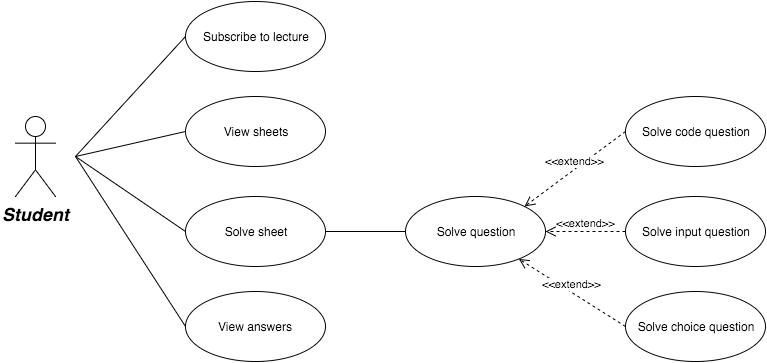
\includegraphics[width=\textwidth,height=\textheight,keepaspectratio]{cases}
	\caption{Use cases for students}
\end{figure}

\begin{figure}[H]
  \centering

	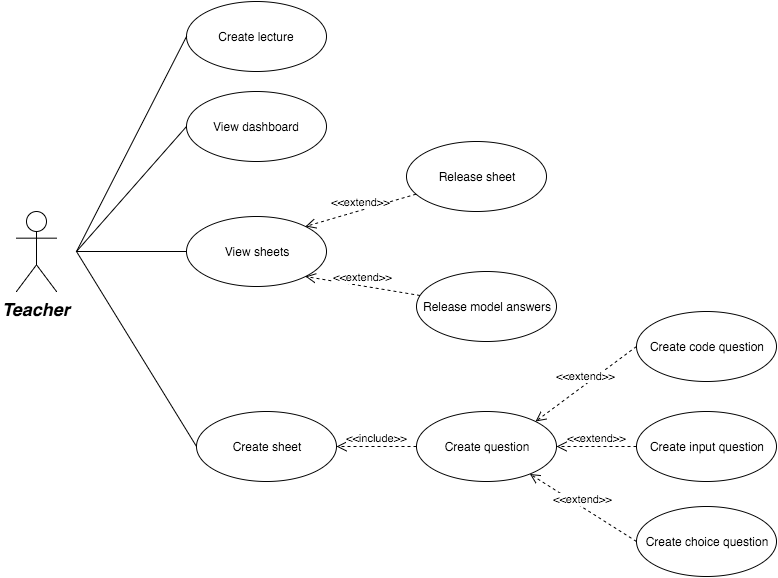
\includegraphics[width=\textwidth,height=\textheight,keepaspectratio]{cases2}
	\caption{Use cases for teachers}
\end{figure}

\subsection{System architecture}
\paragraph{User interface}
Since the user's are assumed to be somewhat technically savvy , the application takes some liberties with having a limited amount of help and information banners since it works similarly to other website the target audience is familiar with.
Overall the application is meant to have a flat design that looks good on any resolution.
Each lecture has a colour chosen by the teacher and shows up throughout the user interface so the user knows which lecture they are looking at.

\subsection{Databases}
There is one database in use which contains all the information relevant to the system , it is located on the same server as the backend ; further in the report you will find some notes on how this can be improved and why.
The database schema is very important since changing it could break parts of the system , it was important to chose a structure that would not drastically change later in the development cycle.
Below is the structure of the tables in the system

\subsubsection{Lecture table}
This table contains all the lectures created

\begin{itemize}
	\item \textit{\textbf{Name}} The name of the lecture , there may be multiple lectures with the same name
	\item  \textit{\textbf{Author}} The teacher who created the lecture , can be any user of the system
	\item  \textit{\textbf{Color}} A Hex , RGB or any valid HTML colour , the current UI allows the teacher to choose a colour from a predefined set. It is used in a number of pages , often used to style all controls on the page - such as buttons or tabs	
\end{itemize}

\subsubsection{Sheet table}
This table contains all the sheets created

\begin{itemize}
	\item  \textit{\textbf{Name}} The name of the sheet
	\item  \textit{\textbf{Lecture ID}} The ID of the lecture this sheet belongs to
	\item  \textit{\textbf{Live}} A boolean that represents whether the students who are subscribed to the lecture can see this sheet ( the teacher can use this to choose when to let the students start completing the sheet)
	\item  \textit{\textbf{Released}} A boolean value that represents if the model answers are released (and the user may no longer change his answers)
\end{itemize}

\subsubsection{Question table}
This table contains all the questions created

\begin{itemize}
	\item  \textit{\textbf{Title}} The body of the question as Markdown formatted text ( stored as plaintext)
	\item  \textit{\textbf{Sheet ID}} The ID of the sheet this question belongs to
	\item  \textit{\textbf{Data}} JSON that provides metadata needed to render the question
	\item  \textit{\textbf{Type}} An integer that defines the type of question
	\item  \textit{\textbf{Correct Answer}} A JSON object that defines metadata needed to compute whether the answer is correct or not	
	\item  \textit{\textbf{Model Answer}} A string that represents an example answer
\end{itemize}

\subsubsection{Answer table}
This table contains all the answers created

\begin{itemize}
	\item  \textit{\textbf{Data}} A plaintext representation of the student's answer
	\item  \textit{\textbf{Question ID}} The question that is answered
	\item  \textit{\textbf{User ID}} The ID of the student who created this answer
	\item  \textit{\textbf{Result}} Plaintext field , used to store the cached computed result of the question.
\end{itemize}

\subsubsection{Statistic table}
This table contains all the statistics created when students answer questions

\begin{itemize}
	\item  \textit{\textbf{Answer ID}} The ID of the answer this statistic is about
	\item  \textit{\textbf{Data}} JSON that contains relevant statistical information about the action
	\item  \textit{\textbf{Kind}} The type of statistic this represents
\end{itemize}



\subsubsection{Subscription table}
This table contains all the subscriptions

\begin{itemize}
	\item  \textit{\textbf{Lecture ID}} The ID of the lecture the user is subscribed to
	\item  \textit{\textbf{User ID}} The ID of the user subscribing to the lecture
\end{itemize}





















